\documentclass[a4paper]{article}   % list options between brackets
\usepackage[utf8]{inputenc}% list packages between braces
\usepackage{microtype} 
\usepackage[T1]{fontenc}
\usepackage[italian]{babel}
\usepackage[babel]{csquotes}
\usepackage[titletoc]{appendix}
\usepackage[style=numeric, backend=bibtex, bibencoding=utf8]{biblatex}
\usepackage{hyperref, amsmath,amssymb, enumerate, indentfirst, booktabs, listings, colortbl, tabularx, graphicx, url, widetable, multirow, subfig}
\usepackage{algorithm}
\usepackage{algorithmicx}
\usepackage{algpseudocode}
\usepackage{rotating}
\usepackage{array}


\newcolumntype{P}[1]{>{\centering\arraybackslash}p{#1}}

\algrenewcommand\algorithmicfunction{\textbf{method}}
\algrenewcommand\algorithmicrequire{\textbf{class}}

\algtext*{EndFunction}

\algnewcommand\algorithmicclass{\textbf{class}}
\algnewcommand\class{\item[\algorithmicclass]}
\algnewcommand\algorithmicmethod{\textbf{method}}
\algnewcommand\method{\item[\algorithmicmethod]}

\makeatother

\bibliography{bibliography}

\begin{document}

\title{Parallelizzazione dell'algoritmo\\di belief propagation\\tramite CUDA.}   % type title between braces
\author{\href{mailto:alessandro.gottoli@studenti.univr.it}{Alessandro Gottoli - VR352595} \\ \href{mailto:fabio.pettenuzzo@studenti.univr.it}{Fabio Pettenuzzo - VR362044}}
\date{\today}    % type date between braces
\maketitle

\vspace{4cm}
\tableofcontents
\pagebreak

%\listoffigures


%\listoftables

\section{Introduzione}             % chapter 1
In questa relazione andremo ad illustrare come abbiamo parallelizzato l’algoritmo di belief propagation su GPGPU. Per ragioni di brevità ci concentreremo solo sulle fasi che abbiamo parallelizzato, delegando una più approfondita descrizione dell’algoritmo ad un’apposita relazione.

%ALE
Per il momento è sufficiente sapere che si tratta di un algoritmo \emph{message passing} che lavora su \emph{junction tree}, cioè una rappresentazione ad albero delle \emph{reti bayesiane}, e ci permette di calcolare i marginali di ogni cricca non compromettendo il calcolo della probabilità congiunta dell'intera rete e in caso di nuova evidenza di propagarla facilmente.

Ogni nodo del junction tree è una cricca massimale delle variabili della rete. Gli archi sono chiamati separatori e nella nostra implementazione vengono individuati tramite l'algoritmo di \emph{kruskal} calcolando l'albero di copertura massimo. Il peso di ogni arco è dato dal numero di variabili che hanno in comune le cricche che collega e l'algoritmo cerca l'albero di peso massimo per rispettare la proprietà di \emph{running intersection}.

Dopo questa fase di trasformazione l'algoritmo associa la tabella di probabilità condizionale di ogni variabile della rete ad una cricca che contiene tutte le variabili che compaiono nella tabella. Moltiplicando tra loro le tabelle associate alla stessa cricca si ottiene una tabella che identifica la tabella dei potenziali per le variabili della cricca e ogni loro configurazione. Queste tabelle vengono identificate come $\psi$. Anche i separatori hanno la loro tabella formata da tutte le configurazioni che possono assumere le variabili in esso contenuto, e inizialmente vengono inizializzate a 1. Queste tabelle le identificheremo come $\phi$.
I messaggi che vengono passati tra due nodi sono proprio le informazioni necessarie per aggiornare queste tabelle.
Le due diverse tabelle da aggiornare compongono le due fasi che abbiamo deciso di parallelizzare.

Supponiamo di aggiornare la tabella di $\psi_2$ partendo dalla tabella del suo vicino $\psi_1$.
La notazione che useremo sarà `*' per identificare la nuova tabella aggiornata.
L'aggiornamento della tabella del separatore $\phi_{1-2}$ viene chiamata \emph{marginalizzazione} e si ottiene facendo la somma di tutti i valori della tabella $\psi_1$ che hanno la stessa configurazione per le variabili del separatore.
\[
\phi_{1-2}^* = \sum_{vars_{\psi_1}/vars_{\phi_{1-2}}} \psi_1
\]

L'aggiornamento della tabella $\psi_2$ viene chiamata \emph{scattering} e si ottiene moltiplicando la stessa $\psi_2$ per il rapporto tra la tabella del $\phi_{1-2}^*$ appena calcolata e quella vecchia $\phi_{1-2}$.
\[
\psi_2^* = \psi_2 \frac{\phi_{1-2}^*}{\phi_{1-2}}
\]

Queste operazioni si prestano abbastanza bene ad ad essere parallelizzate, in quanto il prodotto del numero di stati che possono assumere le variabili all'interno della stessa cricca può raggiungere dimensioni elevate.
% Proprio su queste due fasi abbiamo concentrato il nostro tentativo di parallelizzazione perché possono raggiungere dimensioni elevate, cioè il prodotto del numero di stati che possono assumere le variabili dentro la stessa cricca.
Seguendo l'articolo~\cite{zheng2011belief} abbiamo deciso di parallelizzare sulla dimensione del separatore, dato che ogni elemento della cricca è associato ad una sola configurazione del separatore.

Dato che gli elementi non sono ordinati per favorire queste operazioni si è resa necessaria una fase di preprocessing, che viene applicata in entrambe le versioni (sequenziale e parallela). % che viene applicata sia nella versione sequenziale sia in quella parallela.
Questa fase consiste nel creare in ogni separatore delle tabelle degli indici associate alle tabelle dei potenziali delle cricche collegate dal separatore stesso.
Le tabelle degli indici sono state costruite %in maniera opportuna 
in modo da sfruttare la \emph{coalescenza della memoria}, ossia permettendo a thread aventi id adiacenti di accedere ad indirizzi di memoria adiacenti. Pertanto gli indici dei valori che vengono sommati sono posizionati sempre ad una distanza pari alla dimensione del separatore.

In fase di inizializzazione viene scelta la scheda avente maggior capacità computazionale.\\
Si noti che solo le schede dotate di capacità computazionale maggiore o uguale a {\tt 2.0} (cioè a partire dalla generazione Fermi) supportano efficientemente il tipo di dato {\tt double}, garantendo prestazioni che sono solo la metà rispetto a quelle ottenibili con i valori in singola precisione. 

Prima di lanciare ogni kernel viene invocata la funzione {\tt cudaDeviceSynchronize()}, in modo da evitare conflitti con eventuali altri utilizzatori della macchina.\\
Inoltre a seguito di ogni funzione CUDA viene invocata la funzione {\tt cudaGetLastError()} per rilevare eventuali errori.
Queste funzioni possono comportare un leggero aggravio in termini prestazionali, ma forniscono più garanzie circa la correttezza del codice.

Di seguito analizzeremo le scelte progettuali effettuate supponendo di invocare l'aggiornamento della tabella $\psi_2$ a partire dai dati della tabella $\psi_1$ collegata dal separatore con tabella $\phi_{1-2}$.

\section{Marginalizzazione}

L'input della procedura è rappresentato da:
\begin{itemize}
\item $\psi_1$: la matrice che rappresenta la tabella dei potenziali. \`E composta da valori {\tt double} ed ha dimensione $n \cdot m$, dove $n$ è la dimensione del separatore, cioè la dimensione dell'output che otterremo sommando i valori oppurtuni e che sarà $\phi_{1-2}^*$. Essa è rappresentata come un array di elementi.
\item tabellaIndici di $\psi_1$: una matrice di valori {\tt unsigned int}, anch’essa di dimensione $n \cdot m$ e rappresentata come un array di elementi. Questa tabella si rende necessaria per non dover ricercare in $\psi_1$ gli elementi sa sommare tra loro, e quindi contiene in ogni cella l’indice della tabella dei potenziali del valore di interesse.
\end{itemize}

Un generico elemento in posizione $(i, j)$, dove $i \in [0...m]$ e $j \in [0...n]$,
è pertanto identificato da:

$\psi_1$[ tabellaIndici[ $i \cdot n + j$ ] ]\\
%Siccome le dimensioni di $n$ non sono sempre potenze di 2 e il nostro metodo lavora bene su tali valori si è deciso di costruire comunque tabelle degli indici di tali dimensioni e riempire le posizioni aggiunte con il valore speciale SIZE_MAX e se quindi si trova un valore maggiore della dimensione della tabella $\psi_1$ semplicemente si assegna 0 per non rovinare la sommatoria.
Fanno eccezione gli indici aventi come valore {\tt SIZE\_MAX}. Questi ultimi vengono utilizzati per indicare che in quella posizione non esiste alcun dato da elaborare. \\
Il loro utilizzo sarà più chiaro quando illustreremo le procedure per calcolare la riduzione su GPGPU, per il momento è sufficiente sapere che, per motivi legati all’efficienza, entrambe le tabelle in input e l’array di output hanno una dimensione che è potenza di $2$. Pertanto, nel caso in cui i dati effettivi non siano una potenza di $2$, le tabelle saranno dimensionate secondo la potenza di $2$ successiva e il valore {\tt SIZE\_MAX} servirà per contraddistinguere i dati in eccesso, che non verranno presi in esame durante i calcoli.

L'output della procedura è un array $result$ di dimensione $n$ contenente in ogni cella $j \in [0...n]$: %la somma delle celle 
\begin{equation}
%result[ $j$ ] =  $\sum_{i=0}^{m} \psi_1$ tabellaIndici[ $i \cdot n + j$ ]  \\ dove $j \in [0...n]$.
result[ j ] =  \sum_{i=0}^{m} \psi_1 [ tabellaIndici[ i \cdot n + j ] ]
\end{equation}
% \\ dove $j \in [0...n]$.
Quest’operazione può essere vista come un caso particolare di un’operazione di riduzione dove il risultato ottenuto non è un unico valore contenente la somma di tutti i valori dell’array di partenza, ma un array contenente la somma di alcuni valori, secondo lo schema precedentemente descritto.

\begin{figure}[!h]
%\centering
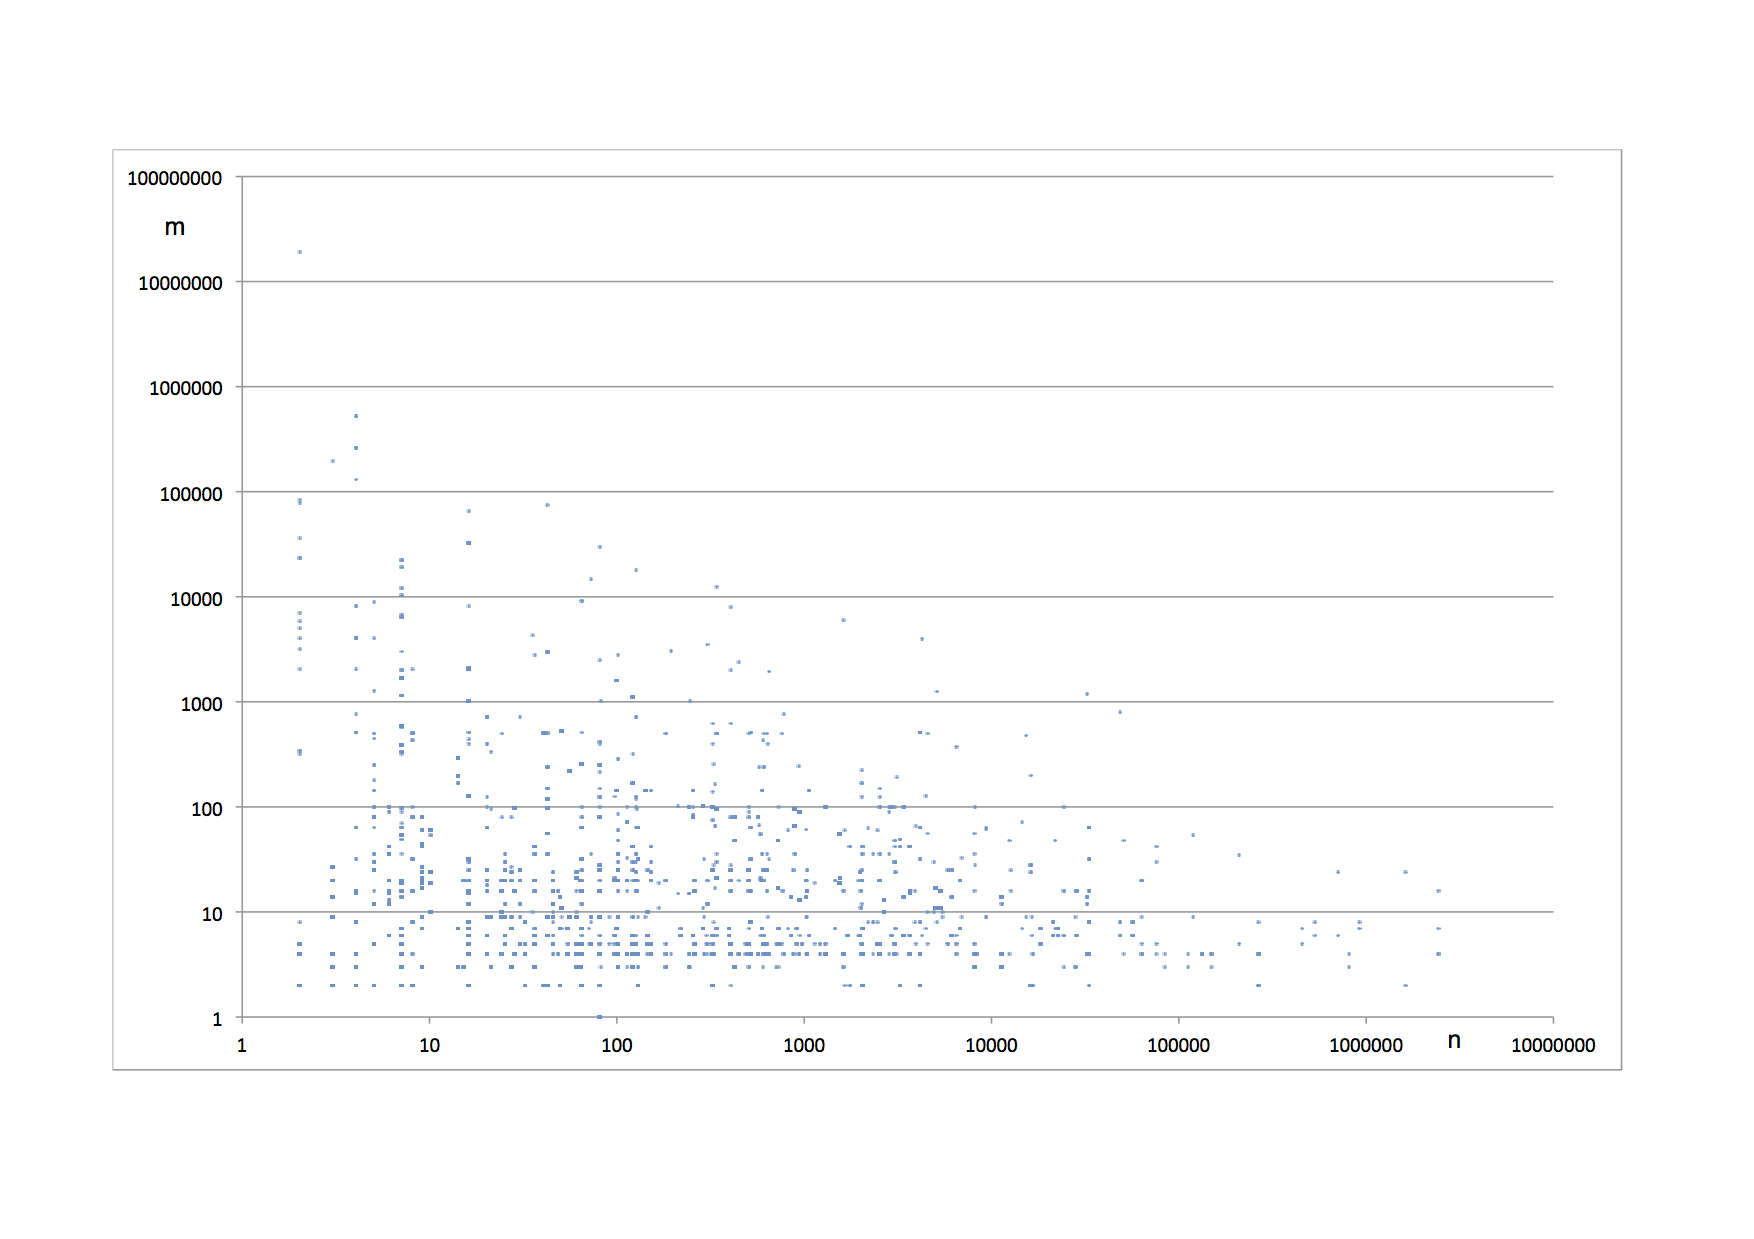
\includegraphics[scale=0.44]{graficoNM.png}
\caption{L'asse delle ascisse rappresenta i valori di n, mentre l'asse delle ordinate rappresenta i valori di m. Entrambi i valori sono su scala logaritmica e relativi ai benchmark su cui sono stati effettuati i test.}
\label{graficoNM}
\end{figure}

 \begin{figure}[!h]
%\centering
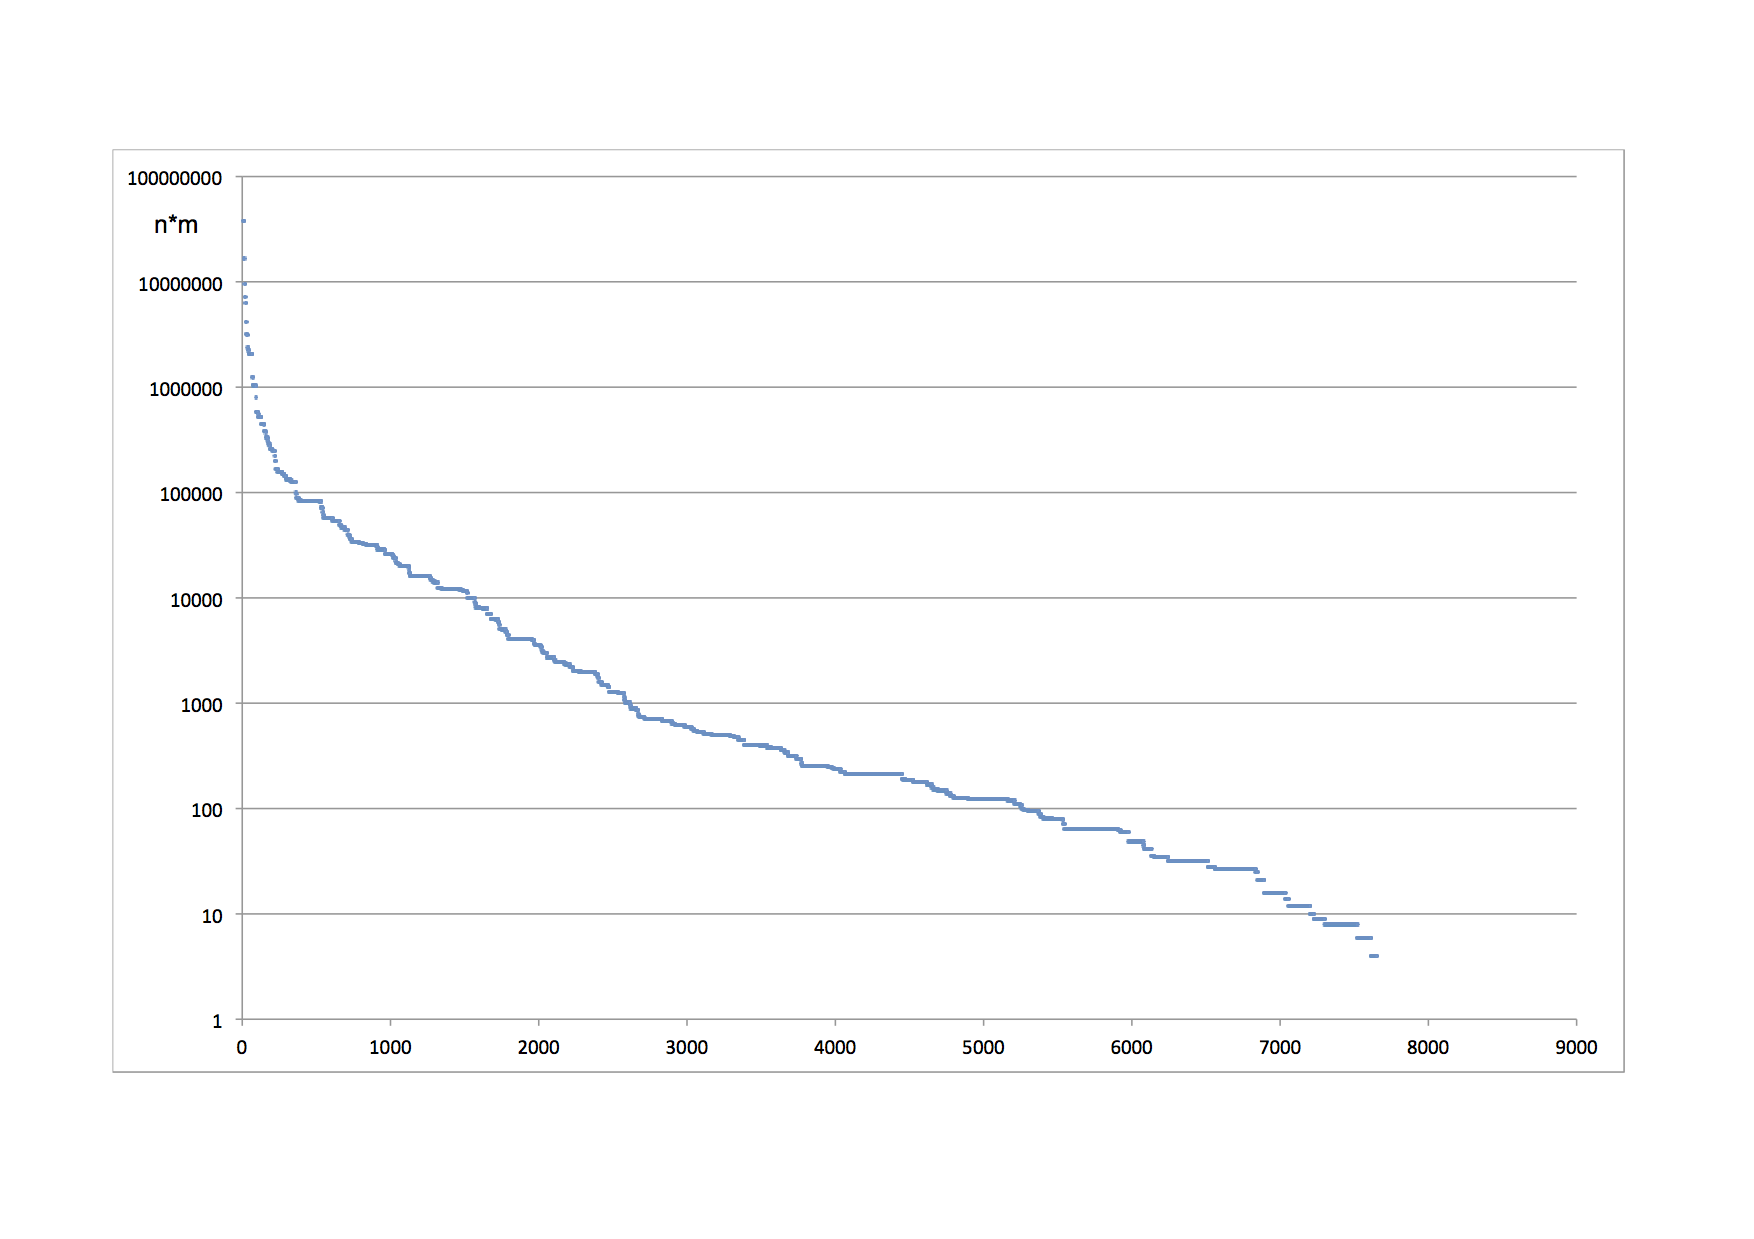
\includegraphics[scale=0.44]{sommavaloretotale.png}
\caption{L'asse delle ordinate rappresenta, per ogni matrice dei benchmark su cui sono stati effettuati i test, la sua dimensione totale secondo una scala logaritmica.}
\label{sommavaloretotale}
\end{figure}

Il metodo è stato implementato da zero in quanto la gestione degli indici non permetteva l’utilizzo di librerie esterne.
Purtroppo le dimensioni dei dati (riportate in Figura \ref{graficoNM} e \ref{sommavaloretotale}) sono estremamente variabili: 
\begin{itemize}
\item vi sono matrici che presentano una delle due dimensioni molto più grande rispetto all’altra
\item vi sono matrici che presentano un buon bilanciamento tra le due dimensioni
\item infine molte matrici presentano dimensioni che rendono sconveniente la parallelizzazione basata su GPGPU.
\end{itemize}
Si rende pertanto necessario uno sviluppo di più approcci, e una precisa definizione dei casi di utilizzo. Di seguito descriveremo gli approcci seguiti, delineando successivamente in che contesto sono risultati più vantaggiosi.

\subsection{Procedura che parallelizza su m}
Il primo approccio vuole andare a coprire i casi in cui $n$ sia un numero piccolo mentre $m$ sia un numero grande. Questo caso è simile ad una riduzione classica, rappresentata dal caso particolare in cui $n$ sia $1$.

 \begin{figure}[!h]
\centering
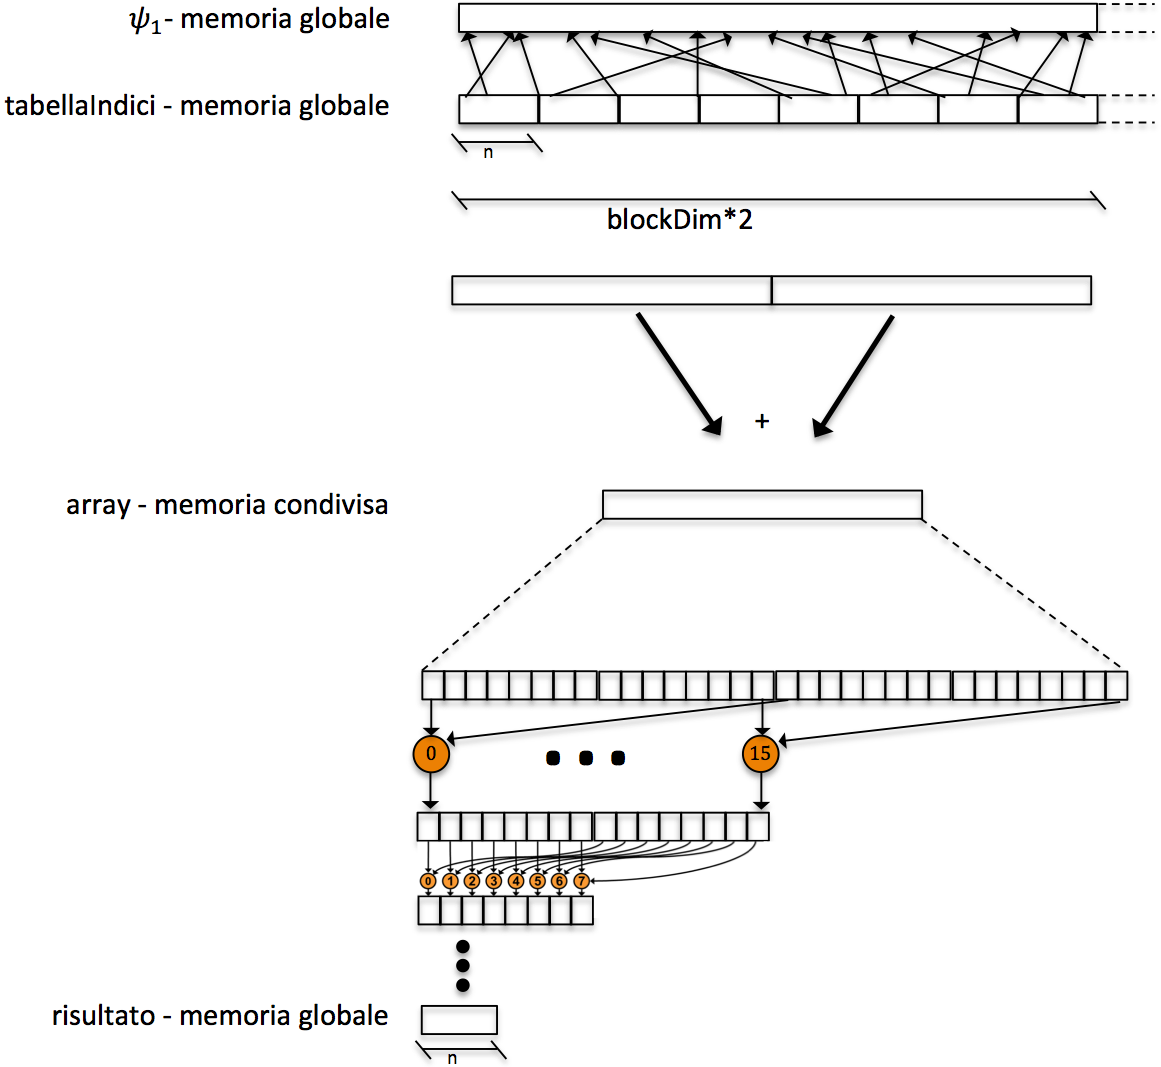
\includegraphics[scale=0.25]{relazionecentrata.png}
\caption{Schema relativo alla marginalizzazione, parallelizzata in funzione di m (fase 1) }
\label{schemafase1}
\end{figure}


L’elaborazione si compone di due fasi, gestite da due kernel appositi:
\subsubsection{Fase 1}
In una prima fase, schematizzata brevemente in Figura \ref{schemafase1}, ogni blocco di thread (di dimensione {\tt blockDim}) legge dalla \emph{memoria globale} un numero doppio di valori rispetto alla sua dimensione. Infatti al suo interno ogni thread legge due valori, posti a distanza {\tt blockDim}, e ne scrive la somma in una cella di un array allocato nella \emph{memoria condivisa}. Il tutto avviene utilizzando la tabellaIndici come sopra descritto.

Così facendo viene effettuata una prima fase di riduzione durante la lettura dalla \emph{memoria globale}, ottimizzando l’utilizzo della \emph{memoria condivisa}. Questa risorsa è preziosa in quanto la riduzione ha una ridotta intensità aritmetica ($1$ flop per ogni elemento caricato) e le sue prestazioni sono pertanto limitate dalla larghezza di banda disponibile. Si noti che ogni valore {\tt double} occupa $8$ Byte, quindi ogni multiprocessore può gestire nella \emph{memoria condivisa} al massimo $6144$ valori.
Inoltre, se non venisse fatta quest’operazione, metà delle threads presenti in ogni blocco verrebbero utilizzate solo per fare una lettura in \emph{memoria globale}. 

Una volta caricate le somme parziali nella \emph{memoria condivisa} il kernel entra in un ciclo il quale, tramite uno shift a destra, dimezza ad ogni iterazione gli elementi da elaborare e le corrispondenti threads.
Ad ogni iterazione ogni thread legge un valore presente nella prima metà degli elementi (corrispondente al proprio {\tt threadId}) e un valore nella seconda metà, sfruttando quindi la \emph{coalescenza della memoria}. Così facendo non si ha \emph{divergenza}, in quanto tutte le thread attive in un blocco hanno id consecutivi e vengono evitati i conflitti tra gli accessi ai banchi di \emph{memoria condivisa}.
Quando il numero di elementi da elaborare è pari a $n$ i valori vengono scritti in \emph{memoria globale}. Per evitare sovrapposizioni tra i risultati scritti da blocchi diversi la scrittura avviene utilizzando un offset dipendente dall’id del blocco in oggetto.

\subsubsection{Fase 2}
La seconda fase si occupa di elaborare i risultati parziali ottenuti dai blocchi nella prima fase, restituendo il risultato finale. 
Seguendo un meccanismo analogo a quello descritto per la prima fase, ogni blocco di thread (di dimensione {\tt blockDim}) legge dalla \emph{memoria globale} un numero doppio di valori rispetto alla sua dimensione. 
Ad ogni iterazione ogni thread legge un valore presente nella prima metà degli elementi (corrispondente al proprio {\tt threadId}) e un valore nella seconda metà. In questo modo viene sfruttata la \emph{coalescenza della memoria} in quanto thread aventi id adiacenti accedono ad indirizzi di memoria adiacenti. Inoltre così facendo non si ha \emph{divergenza}, in quanto tutte le thread attive in un blocco hanno id consecutivi e vengono evitati i conflitti tra gli accessi ai banchi di \emph{memoria condivisa}.

Ogni thread legge quindi due valori, posti a distanza {\tt blockDim}, e ne scrive la somma in una cella di un array allocato nella \emph{memoria condivisa}. In questo caso non è necessario appoggiarsi alla tabellaIndici, in quanto i risultati scritti dalla prima fase sono già ordinati correttamente.
Analogamente a quanto descritto nella fase 1, una volta caricate le somme parziali nella \emph{memoria condivisa} il kernel entra in un ciclo il quale dimezza ad ogni iterazione gli elementi da elaborare e le corrispondenti threads, fino ad ottenere n elementi risultanti. 

Tuttavia, poiché un singolo kernel potrebbe non essere sufficiente per ottenere il risultato finale, questa fase viene iterata fino a lanciare un kernel contenente un solo blocco di thread ed ottenere quindi un array di lunghezza $n$. Il lancio di più kernel in sequenza serve anche come punto di sincronizzazione globale in quanto, per poter procedere nel calcolo, occorre avere la garanzia che tutti i blocchi dell’iterazione precedente abbiano terminato l’esecuzione. Il numero di iterazioni nei casi in esame si mantiene estremamente contenuto ed è in buona sostanza logaritmico nella dimensione dell’input, non comportando dunque un overhead eccessivo. 

%\subsubsection{Ulteriori ottimizzazioni}
\subsubsection{Loop unrolling}
In entrambe le fasi abbiamo scelto di implementare il loop unrolling relativo al ciclo che esegue la riduzione all’interno del kernel. In particolare quanto è attiva un’unica warp, le istruzioni vengono eseguite in modalità SIMD sincrona, procedendo in lockstep. Non è quindi necessario invocare una sincronizzazione esplicita tramite la funzione {\tt \_\_syncthreads()}.

Tuttavia il compilatore potrebbe ordinare le istruzioni di accesso alla \emph{memoria condivisa} inducendo un comportamento non corretto. Ad esempio potrebbe utilizzare i registri (aventi come scope una singola thread) come buffer per ottimizzare le istruzioni store.
In questo caso la \emph{memoria condivisa} è utilizzata come veicolo di comunicazione tra le threads all’interno di un warp, rendendo quindi necessario una redichiarazione del puntatore come {\tt volatile}. In questo modo il compilatore esegue il flushing dei registri ad ogni scrittura, e preleva i dati direttamente dalla memoria senza utilizzare i registri come cache.

Come funzione alternativa abbiamo valutato l’utilizzo di {\tt \_\_threadfence()}, tuttavia abbiamo verificato che, utilizzando questa funzione, veniva aggiunto un overhead inutile se, come nel nostro caso, vi è un unico warp attivo.

Per poter applicare quest’ottimizzazione efficientemente necessitiamo di ridurre al minimo il numero di branch decisi a runtime. Abbiamo dunque utilizzato i template per parametrizzare la dimensione del blocco di thread. Nel codice host uno switch invoca il kernel opportuno in funzione della dimensione scelta a runtime, mentre nel kernel un analogo switch permette di eseguire le corrispondenti istruzioni.

Si noti che questa ottimizzazione fa risparmiare lavoro in tutte le warp, non solo nell’ultima in quanto senza unrolling tutte le warp avrebbero eseguito ogni iterazione del ciclo for, anche se poi non avrebbero partecipato all’aggiornamento dei risultati.

\subsubsection{Istruzioni shuffle}
Un’ulteriore ottimizzazione che abbiamo valutato (ma non implementato) riguarda l’utilizzo delle istruzioni shuffle per permettere uno scambio di valori efficiente all’interno di una warp. Queste istruzioni sono molto utilizzate per eseguire la riduzione di un array nel senso “classico”. Tuttavia nel nostro caso abbiamo degli scambi di valori all’interno di una warp solo quando $n$ è minore di $32$ e solo nelle ultime iterazioni del ciclo interno al kernel. Pertanto abbiamo preferito concentrare i nostri sforzi su altre ottimizzazioni.

\subsection{Procedura che parallelizza su $n$}
Il secondo approccio vuole andare a coprire i casi in cui $m$ sia un numero piccolo mentre $n$ sia un numero grande. \\
Anche in questo caso l’elaborazione si compone di due fasi, gestite da due kernel appositi:
\begin{itemize}
\item In una prima fase ogni blocco di thread (di dimensione {\tt blockDim}) legge dalla \emph{memoria globale} un numero di valori doppio rispetto alla sua dimensione. Infatti al suo interno ogni thread legge un valore nella prima metà degli elementi (in funzione del proprio id e del blocco d’appartenenza) e un valore a distanza $n \cdot m/2$, e ne scrive la somma in \emph{memoria globale}. Il tutto avviene utilizzando la tabellaIndici come descritto in precedenza.
\item La seconda fase si occupa di elaborare i risultati parziali ottenuti dai blocchi nella prima fase, restituendo il risultato finale. Il procedimento eseguito è analogo alla prima fase, con la differenza che in questo caso non è necessario appoggiarsi alla tabellaIndici, in quanto i risultati scritti dalla prima fase sono già ordinati correttamente. 
\end{itemize}
Poiché un singolo kernel potrebbe non essere sufficiente per ottenere il risultato finale, questa fase viene iterata, lanciando ad ogni iterazione un numero inferiore di blocchi, fino a lanciare un kernel contenente un solo blocco di thread ed ottenere quindi un array di lunghezza $n$. 

Il lancio di più kernel in sequenza serve anche come punto di sincronizzazione globale in quanto, per poter procedere nel calcolo, occorre avere la garanzia che tutti i blocchi dell’iterazione precedente abbiano terminato l’esecuzione. Il numero di iterazioni nei casi in esame si mantiene estremamente contenuto ed è in buona sostanza logaritmico nella dimensione dell’input, non comportando dunque un overhead eccessivo. 

In una prima implementazione avevamo realizzato un unico kernel in cui la sincronizzazione tra blocchi era emulata utilizzando le istruzioni atomiche per creare una barriera. Questa soluzione evita l’overhead derivato dalla creazione di nuovi kernel, ma si è dimostrata inadeguata nel caso in cui il numero di blocchi lanciati fosse superiore al numero di blocchi che potevano essere effettivamente schedulati nella GPU. Non potendo garantire la stabilità della soluzione nel caso in cui m fosse eccessivamente grande, abbiamo preferito implementare la soluzione descritta nel paragrafo precedente.

\subsubsection{Dimensionamento dei bloccchi}
In entrambi gli approcci il numero di threads per blocco viene calcolato prima di ogni lancio di kernel. 
\begin{itemize}
\item Se $n \cdot m$, che rappresenta il numero totale di elementi da elaborare, è maggiore o uguale a maxThreads$ \cdot 2$ (in seguito spiegheremo come viene inizializzato maxThreads) il numero di thread allocate è pari a maxThreads.
\item Altrimenti sarà la potenza di $2$ successiva a $(n+1)/2$.
\end{itemize}
Il valore maxThreads ottimale è stato trovato tramite ripetuti test empirici. Abbiamo implementato una procedura che esegue $100$ iterazioni consecutive del kernel, per aumentare la precisione di rilevamento, e ne calcola il tempo medio. La procedura è stata poi eseguita all’interno di $2$ cicli annidati. Il primo itera su tutte le dimensioni (potenze di $2$) delle tabelle in input presenti nei benchmark di riferimento. Il secondo itera su tutte le configurazioni di maxThreads ammesse. Infine per ogni configurazione di input è stata registrato il valore di maxThreads che garantiva prestazioni migliori. 
Il valore di maxThreads che quasi sempre portava a prestazioni migliori è $512$, pertanto abbiamo scelto di lasciare fisso questo parametro.

\subsubsection{Scelta tra i due approcci}
La parallelizzazione su $m$ è molto efficiente, ma si rivela inapplicabile quando $n$ è più grande della dimensione del blocco e le sue prestazioni peggiorano man mano che ci si avvicina a questo limite.
Al contrario, l’approccio che parallelizza su $n$ è utilizzabile, in linea teorica, per elaborare tutti gli elementi. Tuttavia, svolgendo test analoghi a quelli effettuati per determinare il miglior bilanciamento tra threads e numero di blocchi, abbiamo constatato che le prestazioni peggiorano notevolmente in presenza di $m$ grande. 
Dopo aver fatto numerose prove abbiamo deciso di applicare il primo approccio solo quando $n$ è minore di $512$, e il secondo approccio nei restanti casi.

\subsubsection{Utilizzo della memoria costante}
Un’ulteriore ottimizzazione che abbiamo valutato (ma non implementato) per velocizzare la marginalizzazione è quella di utilizzare la \emph{memoria costante} per memorizzare la tabellaIndici e la matrice $\psi_1$. Questa memoria, grazie alla cache, permette di reperire i dati molto più velocemente. 

Tuttavia essendo limitata a $64$KB non è possibile memorizzarvi all’interno più di $5120$ elementi (si noti che ogni elemento occupa $8$ Byte per il valore e $4$ Byte per l’indice). Considerando che per le tabelle di ridotte dimensioni la GPU non porta ad un vantaggio sostanziale, i casi in cui tale soluzione sarebbe applicabile sono un numero relativamente esiguo. Per questo abbiamo preferito concentrarci su altre ottimizzazioni che, a nostro giudizio, possono portare migliori benefici prestazionali.
%\pagebreak
\section{Scattering}
L'input della procedura è rappresentato da:
\begin{itemize}
\item $\psi_2$: la matrice che rappresenta la tabella dei potenziali. \`E composta da valori {\tt double}, ha dimensione $n \cdot m$ ed è rappresentata come un array di elementi.
\item tabellaIndici $\psi_2$: una matrice di valori {\tt unsigned int}, anch’essa di dimensione $n \cdot m$ e rappresentata come un array di elementi. Analogamente a quanto descritto per la marginalizzazione, contiene in ogni cella l’indice della matrice psi del valore di interesse.

Un generico elemento in posizione $(i, j)$, dove $i \in [0...m]$ e $j \in [0...n]$,
è pertanto identificato da: 

$\psi_2$[ tabellaIndici[ $i \cdot n + j$ ] ]\\
Anche in questo caso per elaborare i dati più efficientemente le tabelle sono dimensionate secondo potenze di 2, e viene utilizzata la costante {\tt SIZE\_MAX} nella tabellaIndici per contraddistinguere i dati in eccesso, che non verranno presi in esame durante i calcoli.

\item $\phi^{*}$: è un array di valori {\tt double}, di dimensione $n$
\item $\phi$: è un array di valori {\tt double}, di dimensione $n$
\end{itemize}

%Output della procedura:\\
%$\psi_2$, la matrice ricevuta in input aggiornata come di seguito:\\
%$\psi_2$[ tabellaIndici[ $i \cdot n + j$ ] ] = $\psi_2$[ tabellaIndici[ $i \cdot n + j$ ] ] $ \cdot  \phi^{'}$[ j ]
%dove $\phi^{'}$[ j ] = $\phi^{*}$[ j ] $/ \phi$[ j ]
%e dove $i \in [0...m]$ e $j \in [0...n]$.

L'output della procedura è $\psi_2$, la matrice ricevuta in input aggiornata come di seguito:
\begin{equation}
\psi_2[ tabellaIndici[ i \cdot n + j ] ] = \psi_2[ tabellaIndici[ i \cdot n + j ] ] \cdot  \phi^{'}[ j ]
\end{equation}
dove $i \in [0...m]$, $j \in [0...n]$ e
\begin{equation}
 \phi^{'}[ j ] = \phi^{*}[ j ] / \phi[ j ]
\end{equation}
%e dove $i \in [0...m]$ e $j \in [0...n]$.


L’operazione può quindi essere divisa in due fasi: 

\subsubsection{Fase 1}
La prima fase esegue la divisione elemento per elemento degli array $\phi$ e $\phi^{*}$, aggiornando il valore direttamente in $\phi$.
Sebbene siano presenti molte librerie che eseguono efficientemente simili operazioni per quanto riguarda la somma, non sono state trovate varianti per la divisione. 
Abbiamo pertanto implementato il kernel, allocando per ogni blocco un numero di threads pari a:
\begin{itemize}
\item maxThreads nel caso in cui n (dimensione dell’array) fosse superiore a maxThreads;
\item la potenza di $2$ successiva ad $n$ altrimenti. 
\end{itemize}
Analogamente a quanto descritto nella procedura per il calcolo della marginalizzazione, il valore maxThreads ottimale è stato trovato tramite ripetuti test empirici. In questo caso il valore di maxThreads che quasi sempre portava a prestazioni migliori è 256, pertanto abbiamo scelto di lasciare fisso questo parametro.

\subsubsection{Fase 2}
Durante la seconda fase ogni elemento appartenente alla j-esima riga della matrice psi (recuperato attraverso la tabellaIndici) viene moltiplicato per il corrispondente j-esimo elemento dell'array restituito dalla prima fase. 
La procedura suddivide i blocchi e le threads in modo da avere una threads per ogni elemento della matrice, sfruttando la stessa funzione utilizzata per la prima fase dello scattering.
Anche in questo caso il valore di maxThreads che quasi sempre portava a prestazioni migliori è $256$.
% ( Essendo la matrice psi rappresentata come un array, per moltiplicare ogni elemento con il corrispondente elemento di $\phi^{*}$ viene utilizzata l’operazione modulo. )

\section{Normalizzazione}

L'input della procedura è rappresentato da:\\
${\psi_2}^{*}$: matrice di valori {\tt double} di dimensione $n \cdot m$ ed è rappresentata come un array di elementi.

Output:\\
${\psi_2}^{*}$ normalizzata, ossia in modo che la somma di tutti i suoi elementi sia $1$.

La procedura si può scomporre in due fasi:
\begin{itemize}
\item nella prima fase viene eseguita la somma di tutti gli elementi della matrice.
\item nel caso in cui la somma totale sia diversa da $1$, la seconda fase si occupa di moltiplicare ogni elemento della matrice per un valore costante precedentemente calcolato.
\end{itemize}
Essendo operazioni molto utilizzate esistono diverse librerie che le implementano. Abbiamo quindi effettuato dei test prestazionali utilizzando le librerie Thrust e cuBLAS.
Dai test le cuBLAS si sono rivelate più veloci rispetto alle Thrust, probabilmente a causa del fatto che queste ultime non assumono che ogni riga abbia la stessa lunghezza, e di conseguenza non sfruttino appieno questa regolarità.

\subsubsection{Soglia di parallelizzazione}
Analizzando la figura \ref{sommavaloretotale} si nota come un gran numero di tabelle presenti una dimensione troppo piccola per poter ottere uno speedup positivo dall'elaborazione su GPGPU.
%Per questa ragione abbiamo inserito un controllo che esegue il codice su GPGPU solo nel caso in cui questo risulti essere effettivamente vantaggioso.
Abbiamo pertanto tentato di stabilire una soglia al di sotto della quale elaborare i dati solo su CPU. 

Il controllo viene effettuato sulla dimensione della tabella dei potenziali, prima di eseguire ogni fase di marginalizzazione e di scattering (si noti che a seconda di come procedono le elaborazioni potrebbe risultare conveniente eseguire la marginalizzazione su GPGPU ma non lo scattering, o viceversa).

Mediante misurazioni empiriche abbiamo identificato come $250$ il numero minimo di elementi per cominciare un'elaborazione basata su GPGPU.
Si noti tuttavia che tale valore costituisce solo un'approssimazione in quanto in presenza di piccoli input i tempi misurati risultano essere molto bassi, ed è dunque difficile ottenere misure precise.
Abbiamo inoltre verificato che, dato l’elevato overhead, una volta trasferiti i dati su scheda video è conveniente elaborarli fino alla fine, anche quando questi diventano piccoli.

%, in quanto all'interno dell'algoritmo le stesse tabelle 
%variabile
%In questo caso abbiamo verificato che con matrici che presentavano meno di $250$ elementi il vantaggio ottenuto dalla parallelizzazione su GPGPU non superava l’overhead dovuto ai trasferimenti in memoria e al lancio dei kernel.
%Mediante una procedura analoga abbiamo voluto identificare la dimensione a partire da quale aveva senso elaborare i dati su GPGPU. In questo caso abbiamo verificato che con matrici che presentavano meno di $250$ elementi il vantaggio ottenuto dalla parallelizzazione su GPGPU non superava l’overhead dovuto ai trasferimenti in memoria e al lancio dei kernel.


\section{Test e conclusioni}
% ALE
I test di performance sono stati effettuati su una macchina con cpu Intel Core i7-3770 e gpu NVidia GeForce GTX 680. Le caratteristiche più approfondite si trovano in Tabella~\ref{tab:hw}.

Come benchmark sono state utilizzate le reti presenti nella pagina web \url{http://bndg.cs.aau.dk/html/bayesian_networks.html} (allegate al codice nella directory RetiEsempio).
Per poterle utilizzare è stato costruito un parser che costruisce la rete bayesiana e tutta la procedura di individuazione cricche e costruzione del junction tree per poter applicare l'algoritmo.

Sono state fatte diverse misurazioni per analizzare l'impatto della nostra implementazione parallela, riassunte nella tabella \ref{tab:tempi}.
La tabella è suddivisa in cinque parti:
\begin{itemize}
\item Nella prima parte vengono riportate le caratteristiche delle reti in esame.
\item La seconda parte riporta i tempi totali di esecuzione dell'algoritmo, considerando quindi l'overhead dovuto ai trasferimenti in memoria e al lancio di nuovi kernel.
\item La terza parte riporta i tempi relativi all'esecuzione delle fasi di marginalizzazione e scattering su CPU.
\item La quarta parte riporta i tempi relativi all'esecuzione delle fasi di marginalizzazione e scattering su GPGPU, senza però contare l'overhead dovuto ai trasferimenti in memoria.
\item La quarta parte riporta i tempi relativi all'esecuzione delle fasi di marginalizzazione e scattering su GPGPU, comprensivi dell'overhead dovuto ai trasferimenti in memoria.
\end{itemize}

Come ci si aspettava si hanno risultati migliori al crescere delle dimensioni medie del separatore, tuttavia il tempo trascorso per il trasferimento dei dati tra host e device ci permette di raggiungere risultati equiparabili alla versione sequenziale solo con i benchmark più impegnativi in cui la dimensione media delle tabelle dei separatori è maggiore di 35000. Dai test notiamo che solo l'esecuzione sulla rete Munin1 risulta vantaggiosa, portando uno speedup di $1.44$. %  anche se non di molto.

%Come si può notare il tempo totale di esecuzione dell'algoritmo peggiora per le reti di medio-piccola dimensione. Al contrario la rete più grande, Munin1, porta ad uno speedup di $1.44$.
Quindi siamo passati ad analizzare le prestazioni delle singole fasi (illustrate dalle Figure \ref{graficoMildew}, \ref{graficoDiabetes}, \ref{graficoBarley}, \ref{graficoMunin4}, \ref{graficoWater}, \ref{graficoMunin1}, \ref{graficoLink}) per capire quanta parallelizzazione è possibile ottenere senza considerare l'overhead dovuto ai trasferimenti in memoria.
Nella fase di marginalizzazione il nostro algoritmo si comporta bene in tutte le situazioni, portando lo speedup da un minimo di $2.085$ ad un massimo di $15.75$.
Lo scattering invece è un po' più limitato, ottenendo valori compresi tra $1.029$ e $7.910$.

Le cause dei modesti risultati ottenuti sono a nostro avviso varie:
\begin{itemize}
\item come riportato in Figura \ref{sommavaloretotale} vi sono molti casi in cui la dimensione dei dati è talmente esigua da rendere difficile se non impossibile ottenere uno speedup positivo. 
\item come riportato in Figura \ref{graficoNM} anche in presenza di tabelle di grandi dimensioni, vi sono molti casi in cui è complicato stabilire quale approccio utilizzare per parallelizzare le operazioni, in quanto il rapporto tra le dimensioni è estremamente variabile. % In particolare 
\item inoltre tutte le funzioni implementate sono caratterizzate da una ridotta intensità aritmetica (generalmente $1$ flop per ogni elemento caricato). Come conseguenza le prestazioni sono fortemente limitate dai trasferimenti in memoria. Una possibile soluzione a questo problema è rappresentato dall'utilizzo degli streams, messi a disposizione dall'architettura kepler, ma questa soluzione avrebbe richiesto di ripensare globalmente l'algoritmo per gestire in maniera profondamente diversa le elaborazioni.
\end{itemize}
%Prima di tutto è stato misurato il tempo necessario per l'intera esecuzione della belief propagation per renderci conto se effettivamente si hanno speedup positivi.
%oi si è fatta un'analisi più approfondita delle varie fasi di marginalizzazione e scattering sia considerando il tempo necessario al trasferimento dei dati tra host e device, sia trascurandoli.


%Le misurazioni su alcune reti possono essere viste in Tabella~{\ref{tab:tempi}}.



%i dati ottenuti sono in linea con l'articolo.
Tuttavia confrontandoci con l'articolo \cite{zheng2011belief} possiamo notare come i valori che non tengono conto dell'overhead dovuto ai trasferimenti in memoria siano in linea con i loro risultati.
In particolare nei benchmark Water e Munin4 abbiamo ottenuto risultati migliori; in Mildew e Diabetes abbiamo ottenuto risultati peggiori, mentre con il benchmark Barley i risultati sono complessivamente equivalenti.
A tal proposito è opportuno specificare che:
\begin{itemize}
\item nell'articolo \cite{zheng2011belief} non sono state prese in considerazione le reti Link e Munin1, che con la nostra implementazione garantiscone un notevole speedup.
\item le specifiche tecniche delle macchine, riportate in Tabella \ref{tab:hw} sono notevolmente differenti sia per quanto riguarda la CPU che per quanto riguarda la GPU, rendendo molto difficile un confronto.
\item %Su questi valori abbiamo ottenuto dei risultati simili anche se si nota che ci sono alcune reti che vanno meglio e altre che vanno peggio, questo probabilmente è dovuto anche al fatto che 
se confrontiamo le caratteristiche dei junction tree, esse sono leggermente diverse e ciò e dovuto al metodo (non specificato nell'articolo) utilizzato per la trasformazione della rete bayesiana in junction tree.
\end{itemize}


\begin{table}
\centering
\begin{tabular}{l | l}
\toprule
\multicolumn{2}{c}{\textbf{GPU NVIDIA GeForce GTX 680}} \\
\midrule
\textbf{\# of Processing Cores}	& 1536 \\
\textbf{Shared Memory} &	48K per block \\
\textbf{Global Memory} &	4 GB \\
\textbf{Memory Bandwidth} &	192 GB/sec peak \\
\bottomrule
\multicolumn{2}{c}{} \\
\toprule
\multicolumn{2}{c}{\textbf{CPU	Intel(R) Core(TM) i7-3770 CPU @ 3.40GHz}} \\
\midrule
\textbf{\# of Cores} &	4 \\
\textbf{Processor Clock} &	3.4GHz  \\
\textbf{Cache} &	8 MB \\
\textbf{Memory} &	16 GB \\
\bottomrule
\end{tabular}
\caption{Caratteristiche hardware della macchina su cui abbiamo testato la nostra implementazione.}
\label{tab:hw}
\end{table}


\begin{table}
\small
\centering
\begin{tabular}{ l | r | r | r | r | r | r | r }
%\toprule
\textbf{Dataset} & \textbf{Mildew} & \textbf{Diabetes} & \textbf{Barley} & \textbf{Munin4} & \textbf{Water} & \textbf{Munin1} & \textbf{Link} \\
  \hline
\textbf{\# JT nodes} & 29 & 337 & 36 &  877 & 21 & 162 & 586 \\
  \hline
\textbf{Max CPT size} & 1249280 & 84480 & 7257600  & 448000 & 589824 & 38400000 & 2097152 \\
\hline
\textbf{Min CPT size} & 336 &	495 &	216 &		4	& 9	&	4	& 4 \\

\hline
\textbf{Avg CPT size} & 117257 &	29157 &	476133 &	10102 &	144205	&	516887 &	40928 \\
  \hline
\textbf{Max SPT size} & 62464	& 5280 &	907200 &		56000 &	147456 &		2400000 &	262144 \\
\hline
\textbf{Min SPT size} & 72	& 16 &	7	&	2 &	3	&	2 &	3 \\
\hline
\textbf{Avg SPT size}  & 3950 &	1698	& 38237	&	1376	& 28527 &		58691 &	4418 \\
 \\
%\midrule
%\midrule
\multicolumn{8}{l}{ }	\\
\multicolumn{8}{l}{ }	\\								

\multicolumn{8}{l}{ \textbf{Rilevamenti tempo esecuzione Belief Propagation [ms]:}}	\\		
\hline
\textbf{BP on CPU} & 101 &	275 &	935	&	366 &	152	&	5976 &	1122 \\
\hline
\textbf{BP on GPU} & 693 &	1211 &	978	&		1340 &	318	&	4151 &	1243 \\
\hline
\textbf{Speedup} & 0,146 &	0,227 &	0,956	&	0,273 &	0,478	&	1,440 &	0,903 \\
%\midrule
%\midrule
\multicolumn{8}{l}{ }	\\	
\multicolumn{8}{l}{ }	\\								

\multicolumn{8}{l}{\textbf{Rilevamenti fasi dettagliate [ms]:}} \\
\multicolumn{8}{l}{ }	\\								
\multicolumn{8}{l}{\textbf{Sequenziale:}} \\
\hline
\textbf{marg. on CPU} &	40 & 	98 &	378 &		157 &	63	&	2554 &	492 \\
\hline
\textbf{scatt. on CPU} &	59 &	180 &	511	 &		236 &	83 &		3425 &	692 \\
%\midrule
\multicolumn{8}{l}{ }	\\								

\multicolumn{8}{l}{\textbf{CUDA (senza trasferimenti in memoria)}} \\
\hline
\textbf{marg. on GPU} &	5 &	47 &	32 &	45 &	4 &		213	& 43 \\
\hline
\textbf{scatt. on GPU} &	20 &	175 &	66 &	230 &	14	&	433 &	168 \\
\hline
\textbf{Speedup marg.} & 8 &	2,085 &	11,813 &	3,489 &	15,75	&	11,991 &	11,442 \\
\hline
\textbf{Speedup scatt.} & 2,95 &	1,029 &	7,742 &		1,026 &	5,929 &		7,910 &	4,120 \\
%\midrule
\multicolumn{8}{l}{ }	\\
\multicolumn{8}{l}{ }	\\								

\multicolumn{8}{l}{\textbf{CUDA (con trasferimenti in memoria)}} \\
\hline
\textbf{marg. on GPU} &	210 &	463	& 447 &	430 &	198 &		1458 &	345 \\
\hline
\textbf{scatt. on GPU} &	87	& 550 &	422	& 930 &	74 &		2350 &	808 \\
\hline
\textbf{Speedup marg.} & 0,191 &	0,212 &	0,846 &		0,365 &	0,318 &	1,752 &	1,426 \\
\hline
\textbf{Speedup scatt.} & 0,678 &	0,327 &	1,211 &	 0,254 & 	1,122	&	1,457 &	0,856 \\
%\bottomrule
\end{tabular}
\caption{Statistiche del junction tree (JT) relativi alle reti del dataset, performance della belief propagation (BP) in relazione alle dimensioni delle tabelle dei potenziali delle cricche (CPT) e del separatore (SPT).}
\label{tab:tempi}
\end{table}

\begin{figure}[p]
\centering
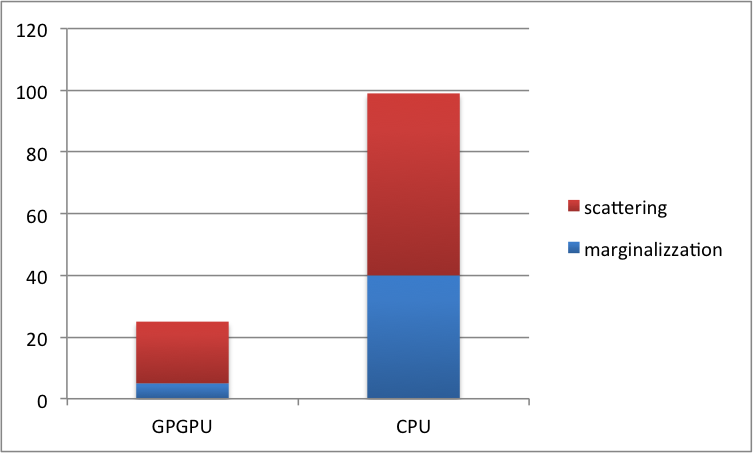
\includegraphics[scale=0.8]{Mildew.png}
\caption{Rete Mildew - tempi misurati in ms.\\Confronto tra CPU e GPGPU (senza considerare i trasferimenti in memoria)} 
\label{graficoMildew}
\end{figure}

\begin{figure}[p]
\centering
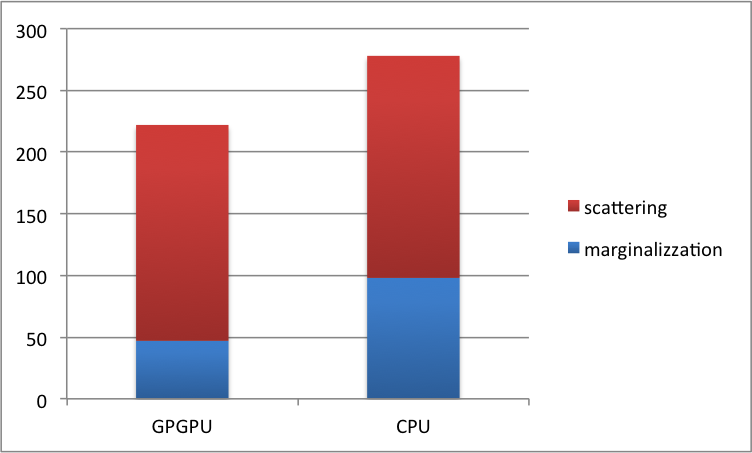
\includegraphics[scale=0.8]{Diabetes.png}
\caption{Rete Diabetes - tempi misurati in ms.\\Confronto tra CPU e GPGPU (senza considerare i trasferimenti in memoria)} 
\label{graficoDiabetes}
\end{figure}

\begin{figure}[p]
\centering
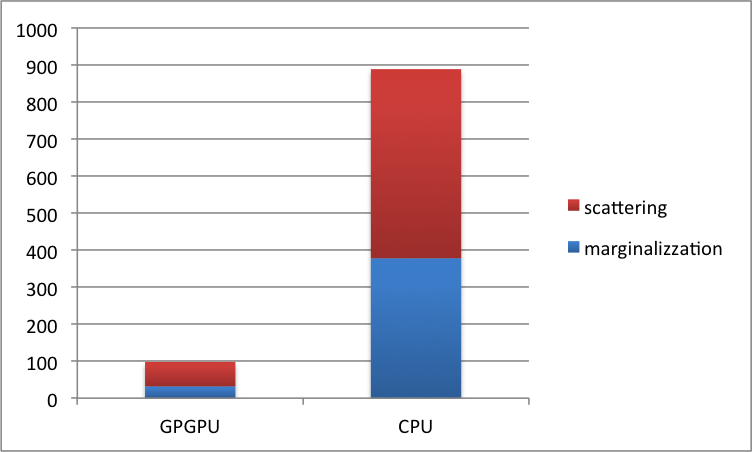
\includegraphics[scale=0.8]{Barley.png}
\caption{Rete Barley - tempi misurati in ms.\\Confronto tra CPU e GPGPU (senza considerare i trasferimenti in memoria)} 
\label{graficoBarley}
\end{figure}

\begin{figure}[p]
\centering
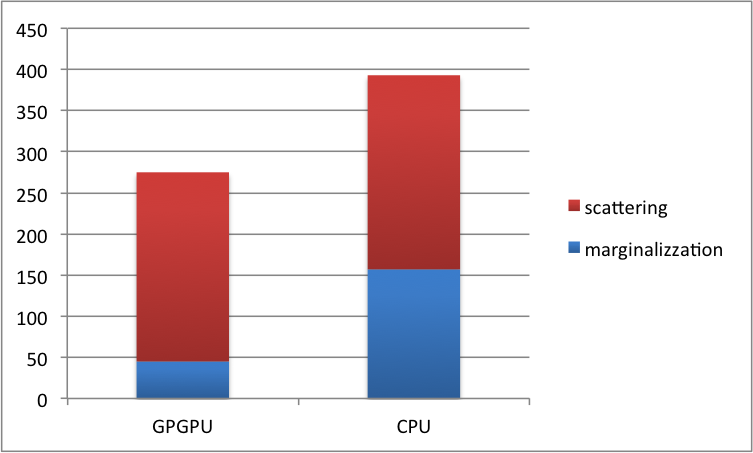
\includegraphics[scale=0.8]{Munin4.png}
\caption{Rete Munin4 - tempi misurati in ms.\\Confronto tra CPU e GPGPU (senza considerare i trasferimenti in memoria)} 
\label{graficoMunin4}
\end{figure}

\begin{figure}[p]
\centering
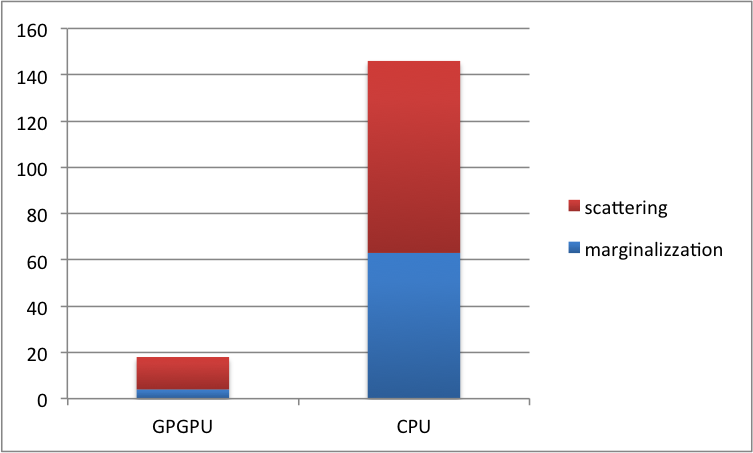
\includegraphics[scale=0.8]{Water.png}
\caption{Rete Water - tempi misurati in ms.\\Confronto tra CPU e GPGPU (senza considerare i trasferimenti in memoria)} 
\label{graficoWater}
\end{figure}

\begin{figure}[p]
\centering
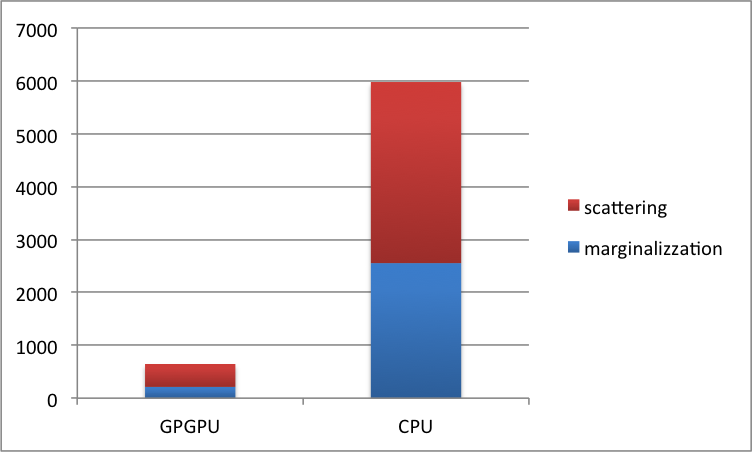
\includegraphics[scale=0.8]{Munin1.png}
\caption{Rete Munin1 - tempi misurati in ms.\\Confronto tra CPU e GPGPU (senza considerare i trasferimenti in memoria)} 
\label{graficoMunin1}
\end{figure}

\begin{figure}[p]
\centering
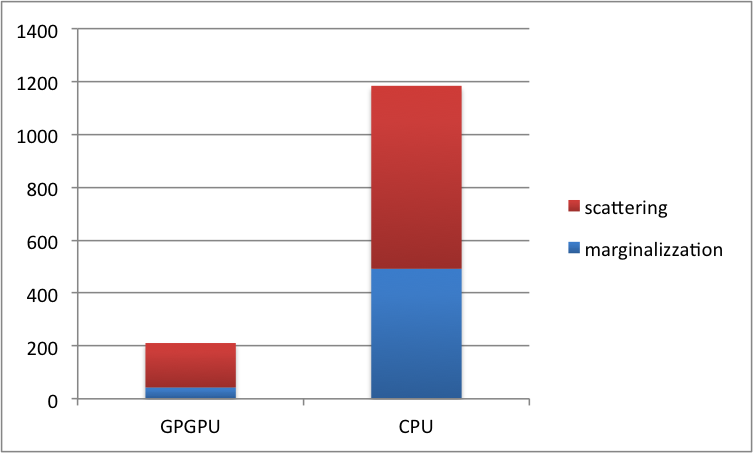
\includegraphics[scale=0.8]{Link.png}
\caption{Rete Link - tempi misurati in ms.\\Confronto tra CPU e GPGPU (senza considerare i trasferimenti in memoria)} 
\label{graficoLink}
\end{figure}

\printbibliography

\end{document}